\documentclass[../Relazione.tex]{subfiles}

\begin{document}
\section{Sensitivity Analysis}
     In questa sezione affronteremo il problema degli \textit{Expired Tickets}. Ognuno di questi comporta una perdita in denaro per il Comune. Il motivo per cui questi ticket scadono è che non vengono gestiti entro un prefissato lasso di tempo (10 giorni) da nessun impiegato (entità \textit{Employee} nella Petri Net), poiché occupato in altre mansioni.
     
     La richiesta è di analizzare i dati raccolti dalle subruns allo scopo di capire se sia conveniente assumere o meno nuovi impiegati (assumendo che l'organico attuale sia di 15 persone) e, nel caso fosse così, quanti bisognerebbe assumerne assumendo che il costo di un impiegato è di \euro400 (\euro2 * 5 giorni * 40 violazioni).
     
     \subsection{Modalità ed Analisi delle Subruns}
         Attualmente il comune, con un organico di 15 persone, in media lascia scadere ticket che, se gestiti, avrebbero portato un guadagno di circa \euro5458, come si evince dal grafico riportato nel \textit{Report Part I}:
         \vspace{0,5cm}
         
         \begin{figure}[!h]
             \centering
             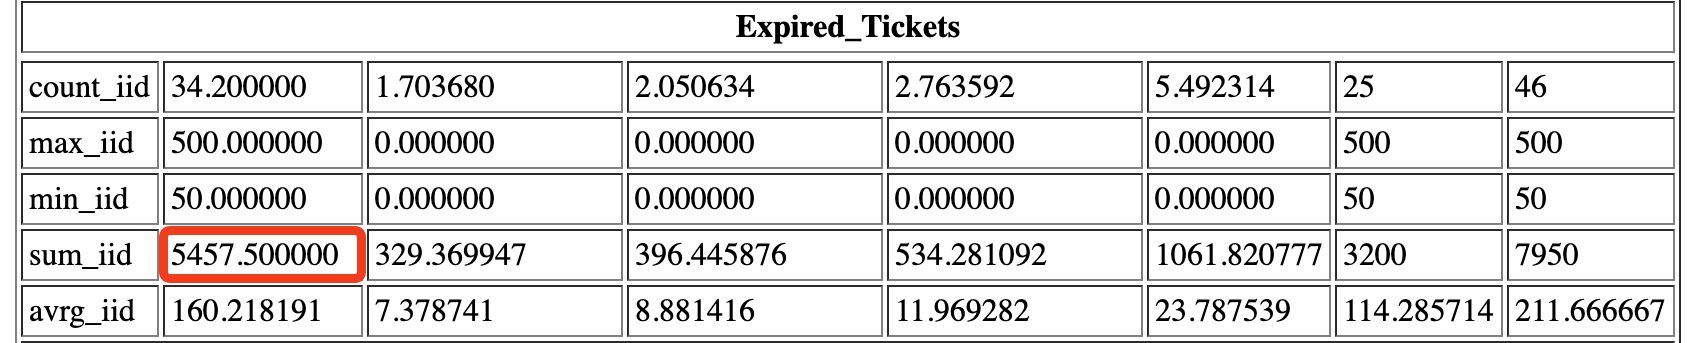
\includegraphics[scale=0.5]{ATCS/simulations/lossPart1.png}
             \caption{\textit{Expired Tickets} con 15 impiegati}
             \label{fig:loss_part1}
         \end{figure}
         \vspace{0,5cm}
         Al fine di massimizzare i guadagni recuperando anche i ticket che scadono, abbiamo effettuato delle simulazioni per prevedere qual è il numero minimo di impiegati da assumere.
         \newpage
         Per rendere più precise queste stime sono state effettuate diverse analisi, \textbf{per ogni nuova assunzione}, secondo lo schema seguente:
         \begin{itemize}
             \item 5 simulazioni da 30 subruns ognuna;
             \item 2 simulazioni da 50 subruns ognuna;
             \item 1 simulazione da 100 subruns.
         \end{itemize}
         
         Di seguito, per praticità, riporteremo solo i valori medi ricavati dalle analisi svolte come descritto precedentemente e riguardanti la somma dei valori degli \textit{Expired Tickets}.
         
         \begin{figure}[!h]
             \centering
             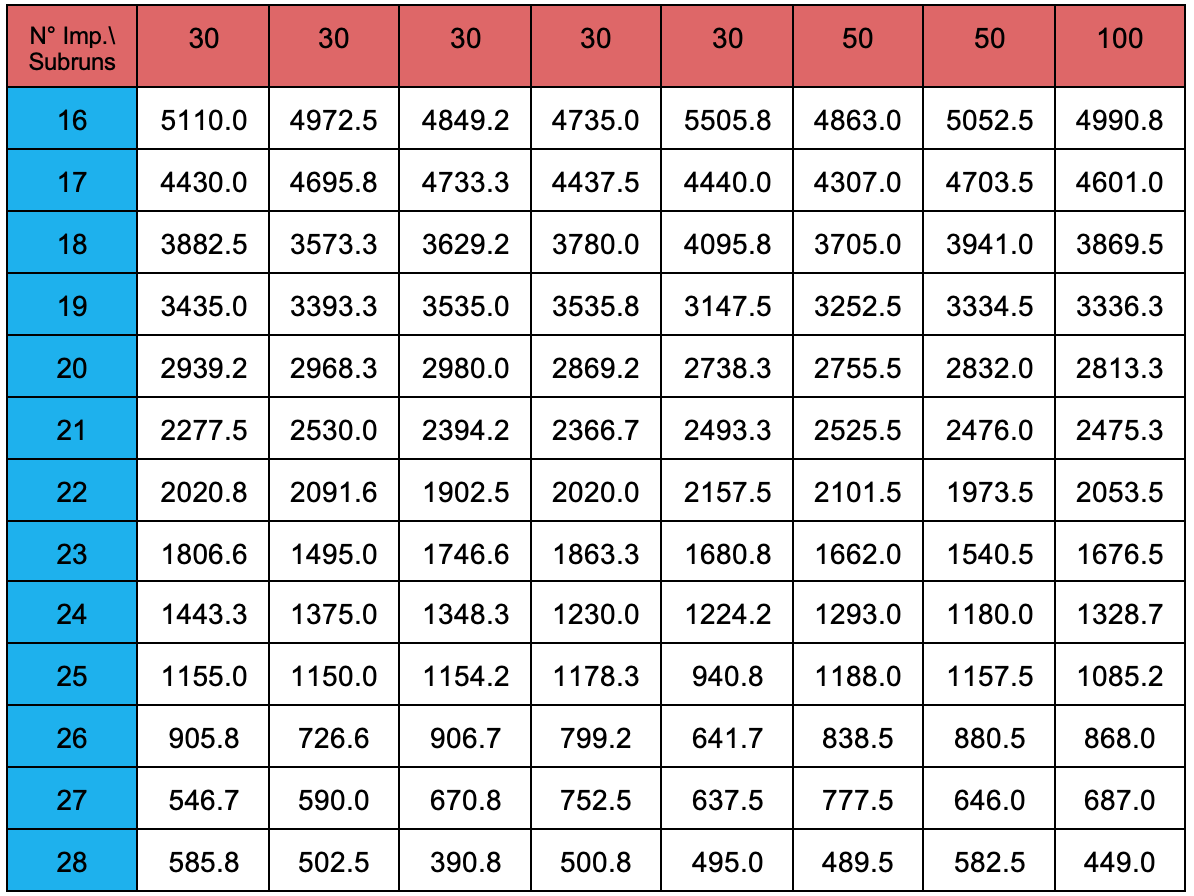
\includegraphics[scale=0.45]{ATCS/figures/runs_avg.png}
             \caption{Valori medi per simulazioni}
             \label{fig:runs_avg}
         \end{figure}
         %\newpage
         \begin{figure}[!h]
             \centering
             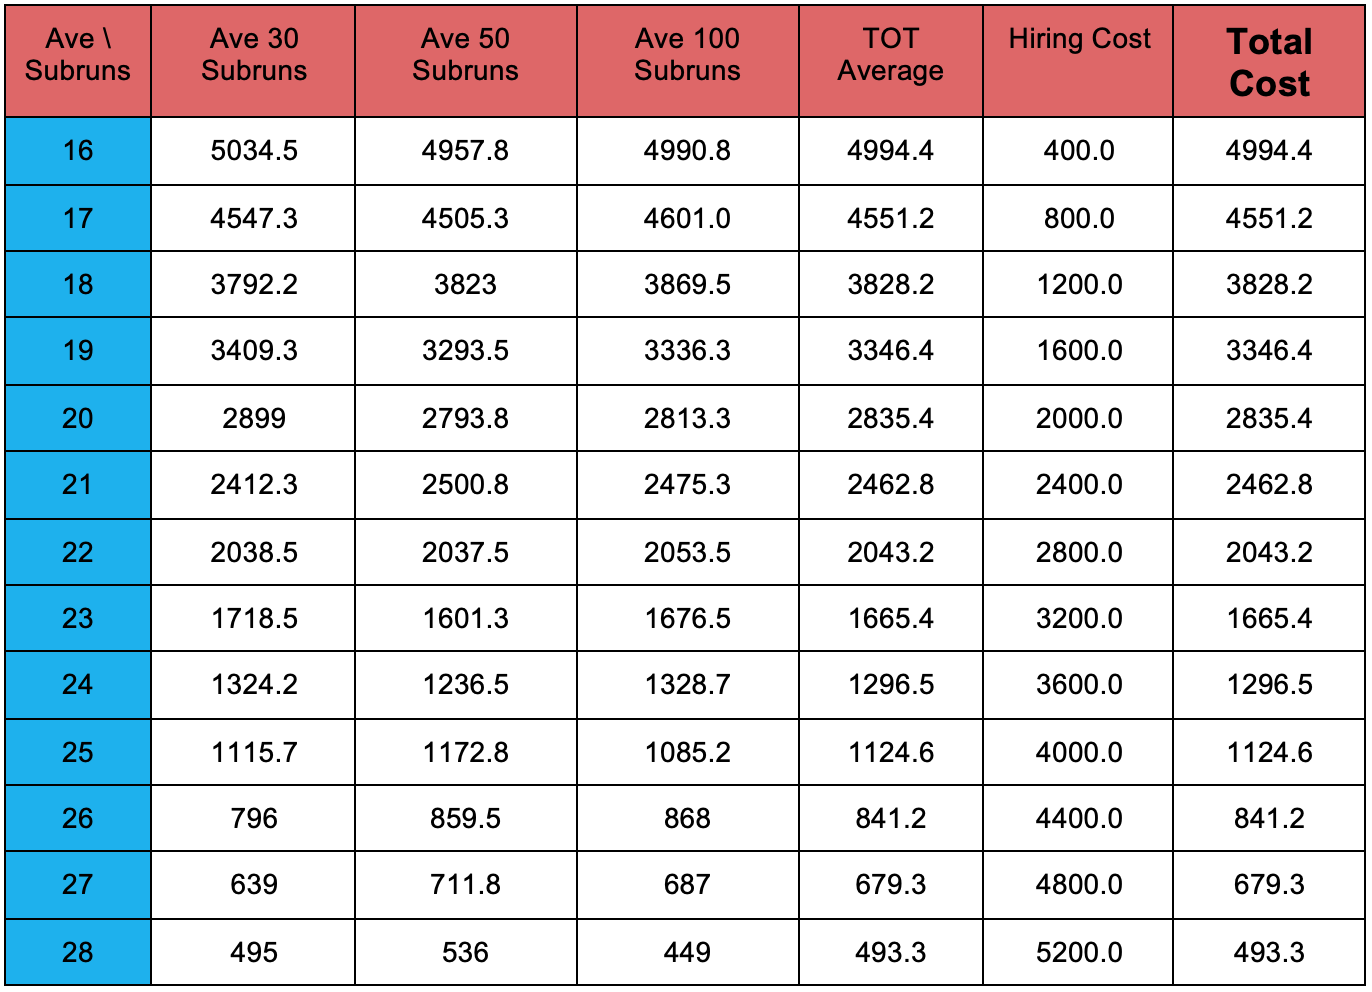
\includegraphics[scale=0.45]{ATCS/figures/tot_avg.png}
             \caption{Medie totali}
             \label{fig:tot_avg}
         \end{figure}
         
\end{document} 
		